\documentclass[a4paper,10pt]{article}

\usepackage{tikz}
\usetikzlibrary{arrows.meta, positioning}
% Add this package to control width
\usepackage[margin=0.8in]{geometry} % 0.8in is a good balance for technical specs



\begin{document}

\title{Testing Automation Suite (TAS)\\Solution and Operating Model}
\author{Internal Working Draft}
\date{\today}
\maketitle

\tableofcontents
\newpage

\section{Purpose and Problem Statement}

The Testing Automation Suite (TAS) exists to enable reliable, repeatable, and explainable regression testing in environments where systems evolve incrementally over time. TAS supports validation of system outputs across successive states, ensuring that changes introduced through code, configuration, or data updates do not result in unintended differences.

Traditional regression testing approaches often rely on manual data extraction, ad-hoc queries, and informal comparison techniques. While such methods can identify differences in isolated cases, they do not scale effectively across systems, releases, or teams. They are prone to inconsistency, difficult to reproduce, and frequently fail to provide clear evidence to support testing outcomes and release decisions.

TAS addresses these limitations by decomposing regression testing into three distinct and coordinated tasks:

\begin{itemize}
  \item Detection of unexpected differences at an aggregate or metric level, providing an early and scalable signal of regression.
  \item Deterministic localisation of discrepancies at record, attribute, or calculation-component level, removing reliance on ad-hoc analysis.
  \item Controlled construction of test expectations derived from documented change intent or requirements, with explicit human oversight and without delegating correctness decisions to automation.
\end{itemize}

Together, these tasks establish a regression testing approach that is incremental by design, scalable across systems, and suitable for consistent application by testing teams operating within a shared Testing Center of Excellence.

In support of expectation-driven testing, TAS treats the construction of tests as a staged process rather than a single automated step. Requirements and change intent are progressively transformed into executable tests through a sequence of constrained activities, each with explicit inputs, outputs, and authority. Assistive automation, including AI, is used only to propose intermediate artefacts; correctness is established through deterministic execution and human validation rather than inferred or assumed.

\section{Scope and Applicability}

This document defines the scope and applicability of the Testing Automation Suite (TAS) as a shared testing capability within the Testing Center of Excellence.

\subsection{In-Scope Usage}

TAS is applicable to regression testing scenarios where system outputs are expected to remain stable across incremental changes, unless an intentional change has been introduced. In-scope usage includes scenarios requiring one or more of the following capabilities:

\begin{itemize}
  \item Comparison of system outputs across successive executions, versions, or states.
  \item Validation of calculated metrics, derived attributes, and aggregated results.
  \item Identification and localisation of unintended differences introduced through system changes.
  \item Support for regression testing across multiple systems, domains, or platforms using a consistent testing approach.
\end{itemize}

These scenarios commonly arise in high-impact systems, including but not limited to finance, risk, regulatory reporting, and other critical business processes.

\subsection{Conditional Usage}

TAS may be applied selectively in the following situations:

\begin{itemize}
  \item Early-stage development or exploratory testing where no stable reference state exists.
  \item One-off analytical investigations not intended to support formal test outcomes.
  \item Prototyping activities where testing intent is still evolving.
\end{itemize}

In such cases, TAS functions primarily as an accelerator rather than a reference testing capability.

\subsection{Out-of-Scope Activities}

TAS does not attempt to automate or replace:

\begin{itemize}
  \item Interpretation of business, policy, or regulatory intent.
  \item Design decisions regarding expected system behaviour.
  \item Exploratory testing aimed at discovering previously unknown behaviours.
\end{itemize}

These activities may inform testing inputs but remain outside the scope of TAS.

\subsection{Applicability Constraint}

Where TAS is applied as the reference regression testing approach, outputs and discrepancies identified by TAS are treated as the baseline for further investigation and decision-making. Alternative analysis techniques may be used to provide explanation or context, but not to invalidate observed results.

\section{Conceptual Model of Testing in TAS}

This section defines the conceptual model that underpins the Testing Automation Suite (TAS). The model describes how testing knowledge is constructed, validated, and used to support reliable regression testing across evolving systems.

\subsection{Testing as Comparison Across System States}

TAS is based on the assumption that systems evolve incrementally over time through changes to code, configuration, data, or infrastructure. Testing, in this context, is concerned with comparing outputs produced by a system in different states in order to identify and explain differences.

Rather than treating regression testing as a single activity, TAS models it as a sequence of related tasks that together establish whether observed differences are expected, acceptable, and correctly implemented. The objective is not only to detect change, but to make change explainable.

\subsection{Separation of Detection, Localisation, and Expectation}

The TAS model separates regression testing into three distinct concerns:

\begin{itemize}
  \item \textbf{Detection}: identifying whether differences exist between system states at an aggregate or summary level.
  \item \textbf{Localisation}: determining precisely where and how those differences manifest within the data.
  \item \textbf{Expectation}: defining what behaviour is intended or acceptable based on documented change intent or requirements.
\end{itemize}

These concerns address different failure modes of traditional testing and require different forms of automation and oversight. Conflating them leads to either missed regressions, excessive manual effort, or untestable assumptions.

\subsection{Testing as a Chain of Constrained Constructions}

TAS treats the construction of tests and test results as a staged process rather than a single automated step. Each stage transforms its inputs into more concrete artefacts through constrained operations, with increasing epistemic authority.

Intermediate artefacts produced during testing—such as structured test intent, executable test cases, or data access logic—are treated as \emph{reviewable hypotheses}. They represent proposed interpretations or implementations of testing intent and are subject to validation, revision, or rejection.

No intermediate artefact is considered authoritative solely by virtue of being generated.

\subsection{Authority Gradient in Testing Artefacts}

Within TAS, different artefacts carry different levels of authority:

\begin{itemize}
  \item Artefacts derived from natural language inputs or change descriptions are inherently interpretative and carry the lowest authority.
  \item Executable test definitions and data access logic carry medium authority once validated, but remain representations of intended checks rather than evidence.
  \item Executed test results produced through deterministic comparison of system outputs carry the highest authority and constitute factual evidence of system behaviour.
\end{itemize}

This authority gradient is fundamental to how TAS incorporates automation, including AI-assisted capabilities, without delegating correctness decisions to probabilistic processes.

\subsection{Role of Automation and Human Oversight}

Automation within TAS is applied selectively based on the nature of the task being performed. Assistive automation may be used to propose interpretations, mappings, or candidate artefacts, but does not assert correctness.

Human oversight is applied at points where interpretation, intent, or acceptance of change is required. Deterministic execution and comparison, once configured and validated, proceed without manual intervention and produce immutable results.

This separation ensures that accountability for meaning and intent remains human, while evidence of system behaviour remains machine-derived.

\subsection{Implications for Regression Testing Practice}

By adopting this model, TAS establishes a testing approach that is:

\begin{itemize}
  \item Incremental, aligning with how systems evolve in practice.
  \item Scalable, by separating coarse-grained detection from fine-grained analysis.
  \item Explainable, by making the construction and validation of testing knowledge explicit.
\end{itemize}

Subsequent sections describe how this conceptual model is realised through the TAS architecture and modules.

\section{TAS Architecture Overview}

The architecture of the Testing Automation Suite (TAS) is derived directly from its conceptual testing model. It is designed to support staged construction of testing artefacts, deterministic execution of comparisons, and controlled incorporation of automation, including AI-assisted capabilities, without conflating interpretation with evidence.

\subsection{Architectural Principles}

TAS architecture is guided by the following principles:

\begin{itemize}
  \item \textbf{Separation of Concerns}: Detection, localisation, and expectation formation are implemented as distinct architectural capabilities.
  \item \textbf{Deterministic Core}: All execution and comparison logic that produces test evidence operates deterministically.
  \item \textbf{Constrained Automation}: Assistive automation is isolated from authoritative execution paths.
  \item \textbf{Incremental Scalability}: The architecture supports progressive deepening of analysis only when required.
\end{itemize}

These principles ensure that TAS remains scalable, explainable, and suitable for consistent use across multiple systems.

\subsection{High-Level Architectural Structure}

At a high level, TAS consists of three coordinated architectural layers aligned to the testing concerns defined earlier:

\begin{itemize}
  \item A \textbf{Detection Layer} responsible for identifying whether differences exist across system states.
  \item A \textbf{Localisation Layer} responsible for analysing and explaining the structure and location of detected differences.
  \item An \textbf{Expectation Construction Layer} responsible for translating documented change intent into executable test definitions.
\end{itemize}

Each layer produces outputs that may serve as inputs to other layers, but no layer substitutes for the responsibilities of another.

\begin{figure}[h!]
\centering
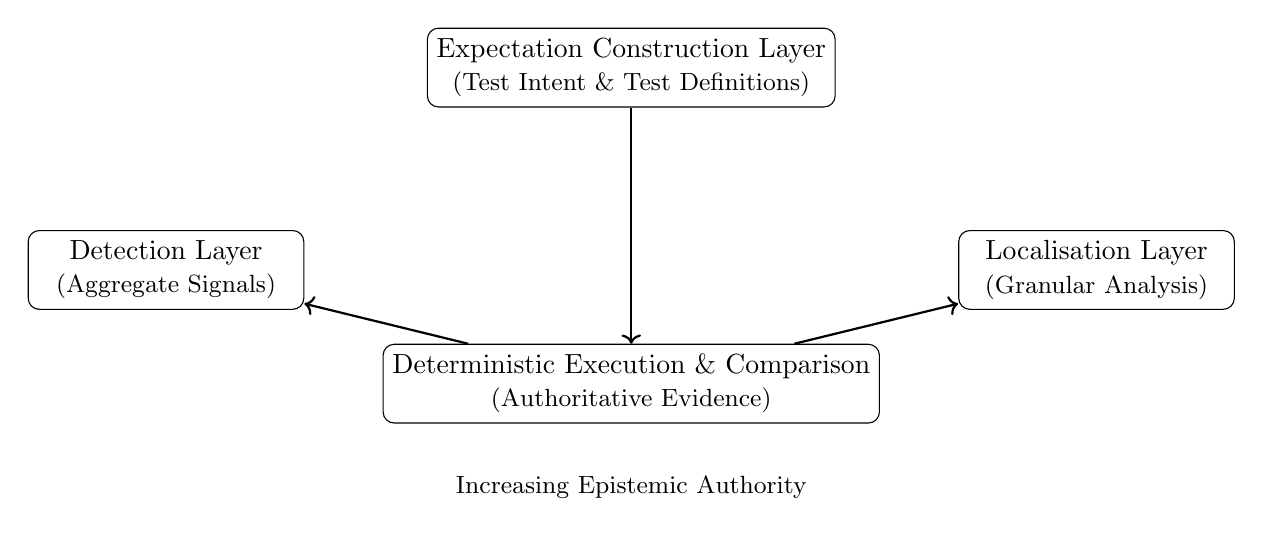
\begin{tikzpicture}[
  node distance=2.2cm,
  every node/.style={draw, rectangle, rounded corners, align=center, minimum width=3.5cm, minimum height=1cm},
  arrow/.style={->, thick}
]

% Layers
\node (expectation) {Expectation Construction Layer\\\small (Test Intent \& Test Definitions)};
\node (detection) [below left=of expectation] {Detection Layer\\\small (Aggregate Signals)};
\node (localisation) [below right=of expectation] {Localisation Layer\\\small (Granular Analysis)};
\node (execution) [below=3cm of expectation] {Deterministic Execution \& Comparison\\\small (Authoritative Evidence)};

% Arrows
\draw[arrow] (expectation) -- (execution);
\draw[arrow] (execution) -- (detection);
\draw[arrow] (execution) -- (localisation);

% Notes
\node[draw=none, below=0.3cm of execution] {\small Increasing Epistemic Authority};

\end{tikzpicture}
\caption{High-Level Architectural Structure and Flow of Evidence in TAS}
\end{figure}

Figure~\ref{fig:architecture-flow} illustrates the high-level architectural structure of TAS. Expectation construction operates upstream, producing hypotheses about intended behaviour. Deterministic execution and comparison form the authoritative core, producing factual evidence of system behaviour. Detection and localisation consume this evidence to support scalable identification and explanation of differences. Assistive automation operates only within the expectation construction layer and does not directly influence execution or evidence generation.


\subsection{Flow of Information and Evidence}

Information within TAS flows through a sequence of transformations with increasing epistemic authority:

\begin{itemize}
  \item Inputs such as system outputs, change descriptions, or requirements enter TAS as raw artefacts.
  \item Intermediate artefacts are constructed to represent hypotheses about expected behaviour or points of difference.
  \item Deterministic execution and comparison produce factual evidence of system behaviour.
\end{itemize}

Only the outputs of deterministic execution are treated as authoritative evidence. Intermediate artefacts remain reviewable and revisable.

\subsection{Isolation of Assistive Automation}

The architecture explicitly isolates assistive automation from authoritative execution paths. Automation may be used to generate candidate artefacts such as structured test intent, test definitions, or data access logic, but these artefacts must pass through validation and review before execution.

This isolation ensures that probabilistic processes do not directly influence test outcomes or evidence generation.

\subsection{Support for Incremental Analysis}

TAS architecture supports incremental analysis by design. Coarse-grained detection may be performed routinely, while fine-grained localisation and expectation-driven validation are invoked selectively based on observed differences or testing objectives.

This approach allows TAS to scale across large datasets and multiple systems without incurring unnecessary computational or operational cost.

\subsection{Technology and Platform Independence}

The TAS architecture is intentionally decoupled from specific technologies, platforms, or tools. While implementations may integrate with particular data stores, requirement repositories, or execution engines, the architectural model does not assume or mandate any specific technology choices.

This abstraction allows TAS to be applied consistently across heterogeneous environments within the Testing Center of Excellence.

\section{TAS Modules}

This section describes the core modules of the Testing Automation Suite (TAS) and their roles within the overall testing model. Each module is defined in terms of the testing task it performs, the nature of its inputs and outputs, and the limits of its authority.

\subsection{DataGuard --- High-Level Regression Detection}

\subsubsection{Purpose}

DataGuard provides an early and scalable mechanism for detecting unexpected differences between successive system states. It operates at an aggregate or metric level and is intended to answer a single question: whether observable outputs have changed in ways that warrant further investigation.

\subsubsection{Testing Task}

The primary task of DataGuard is regression detection. It compares selected summaries, aggregates, or key indicators produced by a system across successive executions or states and identifies deviations beyond defined expectations or tolerances.

DataGuard is designed to be applied routinely and at scale, enabling testing teams to detect potential regressions without incurring the cost of full granular comparison for every change.

\subsubsection{Inputs and Outputs}

Typical inputs to DataGuard include:
\begin{itemize}
  \item Aggregated metrics or summaries derived from system outputs.
  \item Reference values or baselines representing a prior system state.
  \item Comparison rules or tolerances defining acceptable variation.
\end{itemize}

DataGuard produces:
\begin{itemize}
  \item Signals indicating the presence or absence of detected differences.
  \item Structured information identifying which metrics or aggregates exhibit deviation.
\end{itemize}

These outputs may serve as triggers or entry points for more detailed analysis but are not themselves explanations.

\subsubsection{Authority and Limitations}

DataGuard has authority only over the detection of differences at the level it observes. It does not:

\begin{itemize}
  \item Identify the root cause of a detected difference.
  \item Determine whether a detected difference is correct or acceptable.
  \item Provide record-level or attribute-level explanations.
\end{itemize}

A positive signal from DataGuard indicates that further investigation may be required, not that a defect has been confirmed. Conversely, the absence of detected differences at this level does not guarantee that no granular discrepancies exist.

\subsubsection{Role within TAS}

Within the TAS architecture, DataGuard occupies the detection layer. Its role is to provide an efficient and repeatable first pass over system outputs, allowing testing effort to be focused where change is observed.

DataGuard outputs are commonly consumed by localisation capabilities, such as granular comparison, or reviewed in conjunction with expectation-driven testing to determine whether observed differences align with intended change.


\subsection{TrueMatch --- Granular Data Comparison}

\subsubsection{Purpose}

TrueMatch provides deterministic localisation of differences identified during regression testing. It operates at a granular data level and is intended to explain \emph{where} and \emph{how} system outputs differ across successive system states, without interpreting whether those differences are correct or intended.

\subsubsection{Testing Task}

The primary task of TrueMatch is discrepancy localisation. Given two comparable system states, TrueMatch performs structured, repeatable comparison of data at record, attribute, or calculation-component level to identify the precise points at which differences occur.

TrueMatch is invoked when coarse-grained detection is insufficient to explain observed changes, or when detailed evidence is required to support investigation, analysis, or decision-making.

\subsubsection{Inputs and Outputs}

Typical inputs to TrueMatch include:
\begin{itemize}
  \item Comparable datasets or outputs produced by different system states.
  \item Comparison rules defining keys, join conditions, and alignment criteria.
  \item Tolerance definitions for numerical or threshold-based comparison.
\end{itemize}

TrueMatch produces:
\begin{itemize}
  \item Structured listings of discrepancies at record or attribute level.
  \item Categorisation of differences based on type (e.g.\ value change, missing record, additional record).
  \item Supporting evidence sufficient to reproduce the comparison deterministically.
\end{itemize}

The outputs of TrueMatch constitute factual evidence of difference, not conclusions regarding correctness.

\subsubsection{Authority and Limitations}

TrueMatch has authority over the identification and localisation of differences present in the data it compares. It does not:

\begin{itemize}
  \item Interpret business intent or requirement meaning.
  \item Judge whether a difference is acceptable or expected.
  \item Infer root causes beyond the observable structure of the data.
\end{itemize}

TrueMatch operates purely on observable system outputs. Any interpretation of \emph{why} a difference exists or whether it represents a defect lies outside its scope.

\subsubsection{Relationship to Detection and Expectation}

Within the TAS architecture, TrueMatch occupies the localisation layer. It commonly consumes signals from detection capabilities, such as DataGuard, but may also be applied independently when granular evidence is required.

TrueMatch outputs may be reviewed in conjunction with expectation-driven testing artefacts to assess alignment with intended system behaviour. However, such assessment does not alter the factual nature of the discrepancies identified by TrueMatch.

\subsubsection{Role within TAS}

TrueMatch enables testing teams to replace manual, ad-hoc investigation with a repeatable and auditable localisation process. By providing precise and reproducible evidence of how system outputs differ, TrueMatch supports efficient investigation, informed decision-making, and traceable testing outcomes without conflating evidence with interpretation.



\subsection{Test Studio --- Expectation Construction and Test Realisation}

\subsubsection{Purpose}

Test Studio provides a controlled mechanism for constructing testing expectations and executable tests from documented change intent or requirements. Its role is to answer the question of \emph{what should be tested}, without asserting whether a system has behaved correctly.

Test Studio operates upstream of execution and comparison. It produces hypotheses about intended system behaviour that can be evaluated through deterministic testing, rather than conclusions about correctness.

\subsubsection{Testing Task}

The primary task of Test Studio is expectation construction. This involves progressively transforming informal or semi-formal descriptions of change into structured, executable test artefacts that can be evaluated against observed system outputs.

Test Studio does not perform regression detection or discrepancy localisation. Instead, it supplies test definitions and execution logic that may be consumed by other TAS modules to evaluate alignment between intended and observed behaviour.

\subsubsection{Testing as a Chain of Constrained Constructions}

Test Studio is intentionally designed as a sequence of constrained transformations rather than a single automated step. Each stage produces intermediate artefacts that are treated as reviewable hypotheses, not authoritative truth. Authority increases only through validation and deterministic execution.

The stages are described below.

\paragraph{Constructor C1 --- Requirement Formalisation (AI-assisted)}

\begin{itemize}
  \item \textbf{Input}: Documented change descriptions or requirements expressed in natural language.
  \item \textbf{Output}: Structured representations of test intent, including conditions, entities, and invariants.
  \item \textbf{Role of Automation}: Assistive interpretation of language into structured form.
  \item \textbf{Authority}: Low. Outputs are inherently interpretative and subject to review, revision, or rejection.
\end{itemize}

This stage does not establish correctness. It proposes candidate interpretations of intent.

\paragraph{Constructor C2 --- Test Case Generation}

\begin{itemize}
  \item \textbf{Input}: Structured test intent produced by requirement formalisation.
  \item \textbf{Output}: Executable test case definitions expressing the checks to be performed.
  \item \textbf{Role of Automation}: Optional and bounded assistance in structuring test cases.
  \item \textbf{Authority}: Medium. Ambiguities must be resolved or explicitly rejected before progression.
\end{itemize}

At this stage, test cases become explicit hypotheses about system behaviour.

\paragraph{Constructor C3 --- Knowledge Mapping and Data Access Construction}

\begin{itemize}
  \item \textbf{Input}: Executable test case definitions.
  \item \textbf{Output}: Data mappings and data access logic required to evaluate the test cases.
  \item \textbf{Role of Automation}: Suggestive only; proposals require validation.
  \item \textbf{Authority}: Medium, contingent on validation.
\end{itemize}

Automation may propose data access logic, but may not assert its correctness.

\paragraph{Constructor C4 --- Test Execution}

\begin{itemize}
  \item \textbf{Input}: Validated test cases and validated data access logic.
  \item \textbf{Output}: Deterministic test results derived from system outputs.
  \item \textbf{Role of Automation}: None beyond execution.
  \item \textbf{Authority}: High. Outputs constitute factual evidence of observed system behaviour.
\end{itemize}

This stage establishes evidence. Outputs from execution may be consumed by detection or localisation modules.

\paragraph{Constructor C5 --- Result Synthesis and Reporting}

\begin{itemize}
  \item \textbf{Input}: Test definitions and execution results.
  \item \textbf{Output}: Structured summaries, evidence artefacts, and reporting views.
  \item \textbf{Role of Automation}: Summarisation only.
  \item \textbf{Authority}: Reporting. This stage does not alter evidence or outcomes.
\end{itemize}

\subsubsection{Human Oversight and Review}

Human review is required at all stages involving interpretation, intent, or acceptance of hypotheses. Intermediate artefacts may be approved, revised, or rejected, but are not treated as authoritative outcomes.

Once execution has occurred, results are immutable. Human judgment applies only to interpretation of evidence and subsequent decision-making, not to alteration of observed outcomes.

\subsubsection{Role within TAS}

Within the TAS architecture, Test Studio supplies expectation-driven testing capability. It enables testing teams to move from informal change descriptions to repeatable, auditable tests while preserving clear separation between interpretation, execution, and evidence.

By constraining automation and explicitly managing authority, Test Studio allows advanced test construction techniques to be used without compromising determinism, accountability, or explainability.



\section{AI Usage and Human-in-the-Loop Controls}

This section defines how assistive automation, including AI-based capabilities, is used within the Testing Automation Suite (TAS), and how human oversight is applied to preserve determinism, accountability, and explainability.

\subsection{Principles Governing AI Usage}

AI usage within TAS is governed by the following principles:

\begin{itemize}
  \item \textbf{Assistive, Not Authoritative}: AI may propose artefacts or interpretations but does not assert correctness.
  \item \textbf{Explicit Authority Boundaries}: No AI-generated output is treated as evidence or outcome.
  \item \textbf{Human Accountability}: Decisions involving intent, acceptance, or interpretation remain the responsibility of human testers.
  \item \textbf{Deterministic Outcomes}: All test evidence is produced through deterministic execution and comparison.
\end{itemize}

These principles ensure that AI augments testing capability without becoming a source of untraceable or probabilistic decision-making.

\subsection{Permitted Uses of AI}

Within TAS, AI may be applied to the following activities:

\begin{itemize}
  \item Interpreting natural-language change descriptions or requirements into structured representations of test intent.
  \item Assisting in the generation or refinement of executable test case definitions.
  \item Proposing candidate data mappings or data access logic required to evaluate test cases.
  \item Producing summaries or narrative descriptions of test execution results for reporting purposes.
\end{itemize}

In all cases, AI-generated artefacts are treated as hypotheses and are subject to review, validation, or rejection.

\subsection{Prohibited Uses of AI}

AI is explicitly not used for the following purposes within TAS:

\begin{itemize}
  \item Determining whether a test has passed or failed.
  \item Modifying or overriding execution results.
  \item Inferring business intent, regulatory correctness, or acceptability of observed differences.
  \item Making release or approval decisions.
\end{itemize}

Any design or implementation that enables such behaviour is considered outside the scope of TAS.

\subsection{Human-in-the-Loop Control Points}

Human review and oversight are applied at defined points where interpretation or intent is involved. These include:

\begin{itemize}
  \item Review of structured test intent derived from change descriptions or requirements.
  \item Approval or revision of generated test cases prior to execution.
  \item Validation of proposed data mappings and access logic.
  \item Interpretation of test execution results and classification of outcomes.
\end{itemize}

Human reviewers may revise or reject intermediate artefacts but do not alter executed results.

\subsection{Immutability of Execution Evidence}

Once test execution has occurred, the resulting evidence is immutable. TAS does not permit modification, suppression, or reinterpretation of execution results through automation or manual intervention.

Subsequent analysis or decision-making may reference execution evidence but does not alter it.

\subsection{Risk Containment and Failure Modes}

By isolating AI usage to assistive stages and enforcing deterministic execution, TAS limits the impact of potential AI failure modes. Errors in interpretation or artefact generation may result in incorrect hypotheses, but cannot directly produce false evidence or mask observed behaviour.

This containment strategy ensures that failures are detectable, attributable, and correctable without undermining trust in testing outcomes.

\section{Testing Lifecycle and Operating Workflow}

This section describes the typical lifecycle and operating workflow through which the Testing Automation Suite (TAS) is applied in practice. The workflow illustrates how the TAS modules and controls interact to support repeatable and explainable regression testing across evolving systems.

\subsection{Overview of the Testing Lifecycle}

The TAS testing lifecycle spans from the identification of testing intent through to the interpretation of test results. It is structured to ensure that expectations, execution, and evidence are clearly separated, and that testing outcomes can be traced back to documented inputs.

At a high level, the lifecycle consists of the following phases:
\begin{itemize}
  \item Definition of testing intent
  \item Construction of executable tests
  \item Deterministic execution and comparison
  \item Detection and localisation of differences
  \item Interpretation and outcome classification
\end{itemize}

Not all phases are required for every testing scenario; however, the ordering and authority relationships between them are preserved whenever they are applied.

\subsection{Definition of Testing Intent}

The lifecycle begins with the definition of testing intent. This may be derived from documented change descriptions, requirements, or other agreed sources of expected system behaviour.

Where Test Studio is used, this phase includes the formalisation of intent into structured representations that can be reviewed and refined. Outputs from this phase express hypotheses about expected behaviour and do not constitute test outcomes.

\subsection{Construction of Executable Tests}

Structured testing intent is transformed into executable test definitions through controlled construction steps. This includes the definition of test cases, alignment of data elements, and preparation of access logic required for execution.

Intermediate artefacts produced during this phase are subject to review and validation. They are treated as representations of intended checks rather than authoritative evidence.

\subsection{Deterministic Execution and Comparison}

Once test definitions and execution logic have been validated, tests are executed deterministically against system outputs. This phase produces factual evidence of observed system behaviour.

Execution results are immutable and form the authoritative basis for all subsequent analysis. No interpretation or acceptance decisions are applied during this phase.

\subsection{Detection of Differences}

Following execution, detection capabilities may be applied to identify whether observable differences exist across system states at an aggregate or summary level. This phase supports scalable identification of potential regressions and helps prioritise deeper analysis.

Detection outputs indicate the presence or absence of differences but do not explain their nature or cause.

\subsection{Localisation and Analysis}

Where differences are detected or detailed evidence is required, localisation capabilities are applied to identify precisely where and how outputs differ. This phase produces granular, reproducible evidence suitable for investigation and review.

Localisation outputs remain factual and descriptive. They do not assert whether differences are correct, acceptable, or intended.

\subsection{Interpretation and Outcome Classification}

The final phase involves interpretation of execution evidence in the context of documented intent. Human reviewers assess whether observed differences align with expected behaviour, represent acceptable change, or require further action.

Outcome classification may result in acceptance of observed behaviour, identification of defects, or initiation of follow-up activities. This phase does not alter execution evidence, but determines how it is used to inform decisions.

\subsection{Iterative Use and Re-Execution}

The TAS lifecycle supports iterative application. Changes to intent, test definitions, or system behaviour may result in re-execution of tests, with new evidence produced and evaluated.

Each execution cycle is independent and reproducible, allowing testing outcomes to be revisited or revalidated as systems continue to evolve.

\section{Governance and Release Approval Rules}

This section defines how testing outcomes produced by the Testing Automation Suite (TAS) are governed and used to support release and quality-related decisions. It clarifies authority boundaries, decision responsibilities, and the treatment of observed discrepancies without prescribing organisational policy.

\subsection{Principles of Governance}

Governance within TAS is based on the following principles:

\begin{itemize}
  \item \textbf{Evidence Precedes Decision}: All release-related judgments are grounded in observable and reproducible test evidence.
  \item \textbf{Separation of Fact and Judgment}: Detection and localisation of differences are factual activities; assessment of acceptability is a judgment.
  \item \textbf{Explicit Accountability}: Decisions regarding acceptance of observed behaviour are attributable to defined roles, not to tools or automation.
  \item \textbf{Traceability of Rationale}: Decisions are expected to be supported by documented explanation and context.
\end{itemize}

These principles ensure that testing outcomes remain explainable and defensible over time.

\subsection{Treatment of Detected Differences}

Differences identified through TAS execution and comparison are treated as factual observations. They are neither assumed to be defects nor dismissed as expected change without review.

When discrepancies are identified, they become items requiring explanation. Explanation may include alignment with documented change intent, identification of known limitations, or confirmation of unintended behaviour requiring remediation.

\subsection{Authority of Test Evidence}

Execution results and discrepancy evidence produced through deterministic comparison constitute the authoritative record of observed system behaviour. Such evidence is not altered, suppressed, or overridden as part of governance or approval activities.

Alternative analyses or interpretations may be used to contextualise evidence but do not invalidate the existence of observed differences.

\subsection{Decision-Making and Outcome Classification}

Outcome classification is performed by designated human reviewers with appropriate domain and testing context. Based on review of evidence and documented intent, outcomes may include:

\begin{itemize}
  \item Acceptance of observed behaviour as intended or acceptable.
  \item Identification of defects or issues requiring remediation.
  \item Deferral of acceptance pending further analysis or clarification.
\end{itemize}

Outcome classification does not modify test evidence; it determines how evidence is acted upon.

\subsection{Conditions for Acceptance with Differences}

Acceptance of a system state in the presence of detected differences requires an explicit and documented explanation. Acceptable explanations include, but are not limited to:

\begin{itemize}
  \item Alignment with approved change intent or requirements.
  \item Expected behavioural changes resulting from implemented modifications.
  \item Known and documented limitations with an agreed remediation plan.
\end{itemize}

Assertions without supporting rationale or traceability do not constitute sufficient explanation.

\subsection{Escalation and Re-Execution}

Where discrepancies cannot be adequately explained or classified, they may be escalated for further investigation. Changes to intent, test definitions, or system behaviour may result in re-execution of tests, producing new evidence for review.

Each execution cycle remains independent and reproducible, preserving a clear audit trail of observed behaviour and decision rationale.

\section{Evidence, Auditability, and Traceability}

This section describes how the Testing Automation Suite (TAS) produces, preserves, and organises test evidence to support explainable testing outcomes, retrospective review, and auditability.

\subsection{Definition of Test Evidence}

Within TAS, test evidence refers to the artefacts produced through deterministic execution and comparison of system outputs. Test evidence captures observable system behaviour at a specific point in time and serves as the factual basis for testing outcomes and decisions.

Test evidence is distinct from test intent, test definitions, or analytical interpretation. While these may inform execution or decision-making, they do not themselves constitute evidence.

\subsection{Evidence Artefacts}

Typical evidence artefacts produced by TAS include:

\begin{itemize}
  \item Execution results generated from deterministic test runs.
  \item Structured discrepancy outputs identifying observed differences.
  \item Metadata describing execution context, including reference states and comparison parameters.
\end{itemize}

Evidence artefacts are generated automatically as part of test execution and are not manually altered.

\subsection{Immutability and Reproducibility}

Test evidence produced by TAS is immutable. Once generated, evidence artefacts are not modified, overwritten, or selectively suppressed.

Reproducibility is achieved by preserving sufficient contextual information to allow re-execution of tests under equivalent conditions. This includes retention of test definitions, data mappings, and comparison logic associated with the execution.

Immutability and reproducibility together ensure that testing outcomes can be independently verified or revisited at a later time.

\subsection{Traceability Across the Testing Lifecycle}

TAS supports traceability across the testing lifecycle by linking:

\begin{itemize}
  \item Documented change intent or requirements.
  \item Constructed test definitions and execution logic.
  \item Deterministic execution results and discrepancy evidence.
  \item Outcome classification and decision rationale.
\end{itemize}

Traceability does not imply that earlier artefacts determine correctness; rather, it provides context for understanding how testing outcomes were derived.

\subsection{Support for Review and Audit}

The organisation of evidence within TAS enables retrospective review of both observed behaviour and decision rationale. Reviewers can examine what was tested, how it was tested, what was observed, and how outcomes were classified.

TAS does not require special audit-specific processes. The same evidence produced for testing purposes is sufficient to support internal review, assurance activities, or external scrutiny where applicable.

\subsection{Limitations of Evidence}

While TAS provides strong guarantees regarding the integrity and reproducibility of test evidence, it does not guarantee completeness of coverage or correctness of intent. Evidence reflects only what was tested and executed.

Understanding these limitations is essential to avoid over-interpreting test results or assuming assurance beyond the scope of executed tests.

\section{Benefits}

This section describes the benefits of the Testing Automation Suite (TAS) in terms of failure modes it eliminates and capabilities it makes reliable. Benefits are expressed as changes in what testing teams can consistently achieve, rather than as performance claims or efficiency metrics.

\subsection{Reliable Detection of Unintended Change}

TAS enables systematic and repeatable detection of unintended differences as systems evolve. By separating coarse-grained detection from detailed analysis, TAS reduces the risk that regressions go unnoticed due to selective testing, inconsistent queries, or human oversight.

This benefit replaces reliance on individual judgment or ad-hoc investigation with a consistent detection capability that can be applied across systems and releases.

\subsection{Explainable Differences Rather Than Silent Deviations}

Traditional regression testing often identifies that something has changed without providing a clear explanation of how or where. TAS addresses this by providing deterministic localisation of discrepancies, allowing differences to be examined and understood without manual reconstruction.

As a result, differences become explainable artefacts rather than unexplained anomalies, supporting faster and more confident investigation.

\subsection{Clear Separation Between Evidence and Interpretation}

By explicitly separating execution evidence from interpretation and decision-making, TAS reduces the risk of conclusions being influenced by incomplete analysis or implicit assumptions.

Testing outcomes are grounded in immutable evidence, while interpretation remains a documented and attributable human activity. This separation improves clarity, accountability, and trust in testing results.

\subsection{Reduced Dependence on Ad-Hoc Testing Practices}

TAS reduces dependence on informal testing practices such as manual SQL extraction, spreadsheet-based comparison, or unstructured scripts. These practices are difficult to reproduce, scale, or govern consistently across teams.

By providing a shared testing capability, TAS supports more consistent testing practices within the Testing Center of Excellence.

\subsection{Controlled Use of Advanced Automation}

TAS enables the use of advanced automation techniques, including AI-assisted test construction, without delegating correctness decisions to automation. By constraining where automation is applied and how its outputs are treated, TAS allows testing teams to benefit from automation while preserving determinism and accountability.

This controlled approach mitigates common risks associated with opaque or probabilistic testing tools.

\subsection{Improved Traceability and Retrospective Understanding}

Through structured traceability between intent, execution, and outcomes, TAS improves the ability to understand how testing decisions were reached. This benefit supports internal review, knowledge transfer, and long-term maintainability of testing assets.

It also reduces the risk that testing outcomes become disconnected from the context in which they were produced.

\subsection{Scalability Across Systems and Teams}

By standardising core regression testing capabilities and separating concerns across modules, TAS scales across multiple systems, domains, and teams without imposing uniform implementation detail.

This allows the Testing Center of Excellence to provide a consistent testing approach while accommodating heterogeneous environments and evolving system landscapes.

\input{sections/11_implementation}
\section{Roles and Responsibilities}

This section outlines the primary roles involved in the use and operation of the Testing Automation Suite (TAS), along with their responsibilities and decision boundaries. Roles are defined in terms of accountability for testing activities and artefacts rather than organisational hierarchy.

\subsection{Business Tester}

Business Testers are responsible for defining and validating testing intent based on documented change descriptions, requirements, or expected system behaviour.

Key responsibilities include:
\begin{itemize}
  \item Reviewing and refining structured test intent derived from documented sources.
  \item Approving or revising executable test cases prior to execution.
  \item Interpreting test execution evidence in the context of business or domain expectations.
  \item Classifying testing outcomes, including acceptance of observed behaviour or identification of defects.
\end{itemize}

Business Testers do not alter execution results or evidence produced by TAS. Their authority applies to interpretation and outcome classification, not to modification of observed data.

\subsection{Test Engineer}

Test Engineers are responsible for configuring, maintaining, and executing TAS capabilities to ensure reliable and reproducible testing.

Key responsibilities include:
\begin{itemize}
  \item Configuring detection, localisation, and execution capabilities.
  \item Validating test definitions, data mappings, and execution logic.
  \item Ensuring deterministic execution and integrity of test evidence.
  \item Supporting investigation of discrepancies through reproducible analysis.
\end{itemize}

Test Engineers are accountable for the technical correctness and repeatability of testing execution, but do not determine business acceptability of results.

\subsection{System or Application Owner}

System or Application Owners are responsible for providing context regarding system changes and expected behaviour.

Key responsibilities include:
\begin{itemize}
  \item Supplying accurate and timely information regarding system changes.
  \item Clarifying intended behaviour when discrepancies are identified.
  \item Supporting resolution of defects or issues identified through testing.
\end{itemize}

System Owners contribute to explanation and remediation but do not override test evidence.

\subsection{Testing Center of Excellence}

The Testing Center of Excellence (TCoE) is responsible for defining, maintaining, and evolving the TAS operating model.

Key responsibilities include:
\begin{itemize}
  \item Establishing standards and guidance for TAS usage.
  \item Supporting onboarding and adoption across teams.
  \item Reviewing feedback, limitations, and improvement opportunities.
  \item Ensuring consistency of testing practices across systems and domains.
\end{itemize}

The TCoE does not participate in day-to-day outcome classification but provides oversight and stewardship of the testing capability.

\subsection{Governance and Assurance Functions}

\section{Limitations and Known Constraints}

This section documents the known limitations and constraints of the Testing Automation Suite (TAS). These limitations are not defects in the solution, but inherent boundaries of what automated and semi-automated testing can reliably achieve.

Understanding these constraints is essential to avoid over-reliance on TAS outcomes or misinterpretation of testing evidence.

\subsection{Dependence on Defined Scope and Inputs}

TAS operates on the basis of explicitly defined testing intent, test definitions, and comparison criteria. It does not infer what should be tested in the absence of documented inputs.

If testing intent is incomplete, ambiguous, or outdated, TAS may faithfully execute tests that do not fully reflect desired coverage. In such cases, limitations arise from the quality of inputs rather than execution capability.

\subsection{Coverage Is Bounded by Test Definitions}

TAS provides strong guarantees regarding the correctness and reproducibility of executed tests, but it does not guarantee completeness of testing coverage.

Outputs and evidence reflect only what has been explicitly tested. Unspecified behaviours, unmodelled data paths, or omitted scenarios remain outside the scope of observed evidence.

\subsection{Detection Sensitivity Is Configuration-Dependent}

Detection and localisation capabilities depend on the selection of metrics, aggregates, keys, and tolerances. Poorly chosen detection criteria may fail to surface certain classes of regression or may generate excessive noise.

While TAS supports systematic configuration, it does not automatically determine optimal sensitivity for all scenarios.

\subsection{Limitations of Assistive Automation}

AI-assisted capabilities within TAS are intentionally constrained to hypothesis generation and summarisation. As a result:

\begin{itemize}
  \item AI-generated interpretations may be incomplete or incorrect.
  \item AI does not resolve ambiguity without human input.
  \item AI does not validate correctness of generated artefacts.
\end{itemize}

These limitations are mitigated through human review and deterministic execution, but they cannot be eliminated.

\subsection{Interpretation Remains a Human Responsibility}

TAS does not determine business correctness, regulatory compliance, or acceptability of observed behaviour. Such determinations require contextual judgment that cannot be automated reliably.

While TAS provides evidence to support interpretation, it does not replace domain expertise or decision-making responsibility.

\subsection{System and Data Preconditions}

TAS assumes that system outputs are accessible, comparable, and sufficiently stable to support regression testing. In environments with highly non-deterministic behaviour, rapidly changing schemas, or incomplete observability, TAS effectiveness may be reduced.

Such conditions require additional controls or adaptations outside the scope of TAS.

\subsection{Risk of Misuse}

Misuse of TAS can occur if:

\begin{itemize}
  \item Test results are treated as proof of correctness rather than evidence of observed behaviour.
  \item Absence of detected differences is interpreted as absence of risk.
  \item Intermediate artefacts are treated as authoritative without execution.
\end{itemize}

These risks are mitigated through adherence to the conceptual model, governance practices, and role separation defined in this document.

\section{Future Evolution}

This section outlines the principles under which the Testing Automation Suite (TAS) may evolve over time. It does not define a roadmap or commit to specific enhancements. Instead, it describes how TAS can be extended while preserving the conceptual, architectural, and governance constraints defined in this document.

\subsection{Principles for Evolution}

Any evolution of TAS is expected to adhere to the following principles:

\begin{itemize}
  \item \textbf{Preservation of Authority Boundaries}: Extensions must not blur the separation between hypothesis generation, deterministic execution, and human judgment.
  \item \textbf{Compatibility with Existing Evidence}: New capabilities must not invalidate or reinterpret previously produced test evidence.
  \item \textbf{Incremental Adoption}: Enhancements should be introducible without requiring wholesale changes to existing testing practices.
  \item \textbf{Explainability by Design}: New features must be explainable within the existing conceptual model rather than introducing opaque behaviour.
\end{itemize}

These principles ensure continuity and trust as TAS evolves.

\subsection{Extension of Testing Capabilities}

Over time, TAS may be extended to support additional forms of regression testing, comparison strategies, or analysis techniques. Such extensions may include broader coverage of data structures, alternative comparison semantics, or enhanced reporting views.

Any extension is expected to integrate with the existing detection, localisation, and expectation construction model rather than replacing it.

\subsection{Evolution of Assistive Automation}

Assistive automation capabilities, including AI-based techniques, may evolve in scope or sophistication. However, such evolution remains constrained by the same rules that apply today:

\begin{itemize}
  \item Automation proposes artefacts; it does not assert correctness.
  \item Deterministic execution remains the sole source of test evidence.
  \item Human oversight remains essential where interpretation or acceptance is required.
\end{itemize}

Improvements in automation are intended to reduce manual effort and increase consistency, not to alter authority or accountability.

\subsection{Adaptation to Changing System Landscapes}

As system architectures, data platforms, and delivery practices evolve, TAS may be adapted to operate effectively within new environments. Such adaptation focuses on maintaining conceptual consistency rather than enforcing uniform implementation detail.

The TAS operating model is designed to remain applicable across heterogeneous systems and is expected to evolve in response to organisational learning and experience.

\subsection{Non-Binding Nature of This Section}

This section is informational rather than prescriptive. It does not obligate adoption of specific enhancements or define timelines for change. Decisions regarding future evolution of TAS are expected to be informed by usage experience, organisational priorities, and Testing Center of Excellence governance processes.


\end{document}
